\begin{figure}
\begin{center}
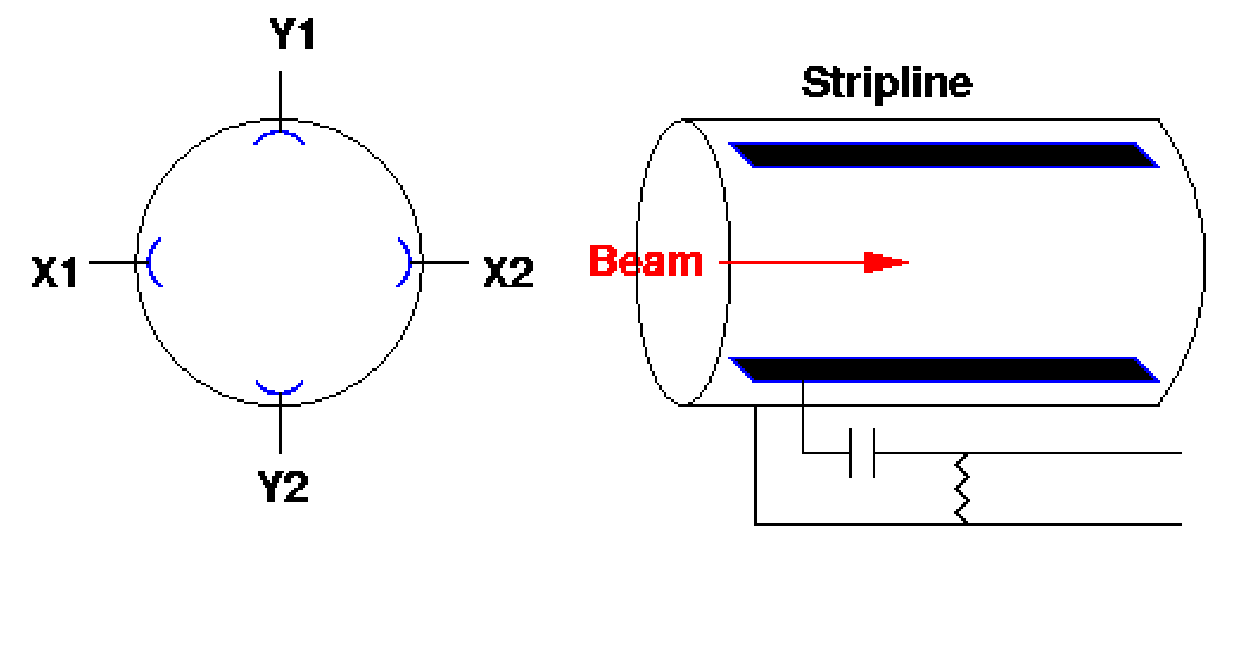
\includegraphics[width=1.0\linewidth]{./figures/bpm_schematic}
\caption{ Beam Current induces a time dependent voltage proportional to the derivative of
the beam current itself. BPM electronics use a comparator circuit, and the readings from
X1/2 and Y1/2 to determine the X and Y beam positions. The absolute measurement of beam
position is subject to offsets stemming from various effects, however, relative positions
(say of one beam to another) are reliable.~\cite{kawallfocus2005}}
\label{fig:bpm_schematic_cartoon}
\end{center}
\end{figure}
